\documentclass[11pt,a4paper]{article}

% ---------------------------------------------------------------------------
%  Encodage, langue, polices
% ---------------------------------------------------------------------------
\usepackage[utf8]{inputenc}
\usepackage[T1]{fontenc}
\IfFileExists{french.ldf}{\usepackage[french]{babel}}{}
\usepackage{helvet}
\renewcommand{\familydefault}{\sfdefault}
\usepackage{courier}

% ---------------------------------------------------------------------------
%  Mise en page
% ---------------------------------------------------------------------------
\usepackage[margin=2.2cm]{geometry}
\usepackage{xcolor}
\usepackage{enumitem}
\usepackage{fancyhdr}
\usepackage{tikz}
\usetikzlibrary{positioning,arrows.meta,shapes.geometric,calc}
\usepackage[edges]{forest}
\usepackage[most]{tcolorbox}
\usepackage{listings}
\usepackage[hidelinks]{hyperref}

\setlength{\parindent}{0pt}
\setlength{\parskip}{0.6em}
\setlist{itemsep=0.25em,topsep=0.3em}

% Couleurs reprises de l'écran GAME OVER
\definecolor{nuit}{RGB}{13,2,34}
\definecolor{magenta}{RGB}{230,35,105}
\definecolor{cyan}{RGB}{40,170,200}
\definecolor{pale}{RGB}{209,248,255}
\definecolor{rouge}{RGB}{200,20,30}
\definecolor{vert}{RGB}{20,140,70}
\definecolor{fondcode}{RGB}{246,244,250}

\pagestyle{fancy}
\fancyhf{}
\fancyhead[L]{\small\color{gray}TP -- Livre dont vous êtes le héros}
\fancyhead[R]{\small\color{gray}IMAMI}
\fancyfoot[C]{\small\thepage}
\renewcommand{\headrulewidth}{0.4pt}

% Titres de sections colorés
\makeatletter
\renewcommand\section{\@startsection{section}{1}{0pt}{1.6em}{0.8em}%
  {\Large\bfseries\color{nuit}}}
\renewcommand\subsection{\@startsection{subsection}{2}{0pt}{1.2em}{0.5em}%
  {\large\bfseries\color{magenta}}}
\makeatother

% ---------------------------------------------------------------------------
%  Code Python
% ---------------------------------------------------------------------------
\lstdefinestyle{python}{
  language=Python,
  basicstyle=\ttfamily\small,
  keywordstyle=\color{magenta}\bfseries,
  commentstyle=\color{gray}\itshape,
  stringstyle=\color{cyan!70!black},
  showstringspaces=false,
  columns=fullflexible,
  keepspaces=true,
  breaklines=true,
  upquote=true,
  literate={é}{{\'e}}1 {è}{{\`e}}1 {ê}{{\^e}}1 {à}{{\`a}}1 {â}{{\^a}}1
           {ç}{{\c{c}}}1 {ù}{{\`u}}1 {û}{{\^u}}1 {î}{{\^i}}1 {ô}{{\^o}}1
           {É}{{\'E}}1 {À}{{\`A}}1 {È}{{\`E}}1 {œ}{{\oe}}1
}
\lstset{style=python}

\newtcblisting{code}{
  listing only,
  colback=fondcode, colframe=nuit!60, boxrule=0.5pt, arc=2pt,
  left=6pt, right=6pt, top=2pt, bottom=2pt,
  listing options={style=python}
}

\newcommand{\guil}[1]{\guillemotleft~#1~\guillemotright}
\newcommand{\fichier}[1]{\texttt{\color{nuit}#1}}

% ---------------------------------------------------------------------------
%  Encadrés
% ---------------------------------------------------------------------------
\newtcolorbox{attention}[1][Attention]{
  enhanced, breakable, colback=rouge!6, colframe=rouge, boxrule=1.2pt, arc=3pt,
  fonttitle=\bfseries\large, title={\raisebox{-1pt}{\Large$\triangle$}\ \ #1},
  left=8pt, right=8pt
}
\newtcolorbox{astuce}[1][Astuce]{
  enhanced, breakable, colback=cyan!6, colframe=cyan!80!black, boxrule=0.8pt, arc=3pt,
  fonttitle=\bfseries, title={#1}, left=8pt, right=8pt
}
\newtcolorbox{convention}[1]{
  enhanced, colback=pale!35, colframe=magenta, boxrule=2pt, arc=4pt,
  fonttitle=\bfseries\Large, coltitle=white, colbacktitle=magenta,
  title={\hfill #1 \hfill}, left=10pt, right=10pt, top=6pt, bottom=6pt
}
\newtcolorbox{consignes}{
  enhanced, breakable, colback=rouge!4, colframe=rouge, boxrule=2pt, arc=4pt,
  fonttitle=\bfseries\Large, coltitle=white, colbacktitle=rouge,
  title={\hfill CONSIGNES OBLIGATOIRES \hfill},
  left=10pt, right=10pt, top=6pt, bottom=6pt
}

% ===========================================================================
\begin{document}
\thispagestyle{empty}

% ---------------------------------------------------------------------------
%  Bandeau de titre
% ---------------------------------------------------------------------------
\begin{tikzpicture}[remember picture, overlay]
  \fill[nuit] ($(current page.north west)+(0,-1.2)$) rectangle
              ($(current page.north east)+(0,-5.6)$);
  \fill[magenta] ($(current page.north west)+(0,-5.6)$) rectangle
                 ($(current page.north east)+(0,-5.8)$);
  \node[anchor=west, text=pale, font=\Huge\bfseries] at
       ($(current page.north west)+(2.2,-2.8)$) {Livre dont vous êtes le héros};
  \node[anchor=west, text=cyan!60!white, font=\Large] at
       ($(current page.north west)+(2.2,-3.9)$) {TP de programmation Python -- un jeu en pages};
  \node[anchor=west, text=magenta, font=\ttfamily\large] at
       ($(current page.north west)+(2.2,-4.8)$) {> python moteur.py histoire\_A12\_};
\end{tikzpicture}
\vspace*{4.2cm}

% ---------------------------------------------------------------------------
\section{Le principe}

Dans un \emph{livre dont vous êtes le héros}, le lecteur ne lit pas les pages dans l'ordre :
à la fin de chaque paragraphe, il fait un choix (\guil{Pour ouvrir la porte, allez page 12 ;
pour fuir, allez page 7}). Vous allez écrire un jeu qui fonctionne de la même façon.

Le thème est \textbf{libre} : aventure, enquête policière, escape game, exploration
spatiale, histoire interactive\dots{} Tout jeu convient, du moment qu'il respecte le
fonctionnement décrit ci-dessous.

\begin{itemize}
  \item Chaque \textbf{page} de votre histoire est une \textbf{fonction Python} écrite
        dans son propre fichier.
  \item Une page affiche du texte, pose éventuellement une question au joueur, puis
        \textbf{retourne le numéro de la page suivante}.
  \item Les informations du jeu (par exemple nom du joueur, points de vie, inventaire,
        indices trouvés, score\dots{}) sont rangées dans un \textbf{dictionnaire} appelé \texttt{gameState}, qui est
        transmis d'une page à l'autre.
  \item Toutes vos fonctions sont \textbf{typées} : on précise le type de chaque
        paramètre et celui de la valeur retournée.
  \item Avant la page 1, une fonction \texttt{menu()} \textbf{prépare la partie} et crée
        le dictionnaire \texttt{gameState} : création d'un personnage, choix d'un niveau
        de difficulté, présentation des règles\dots{} selon ce dont votre jeu a besoin.
\end{itemize}

Votre travail consiste \textbf{uniquement} à écrire la fonction \texttt{menu()}, les
fonctions \texttt{pageX(gameState)} et, si vous le souhaitez, des dessins en ASCII art et
des fonctions annexes (combats, énigmes\dots).

% ---------------------------------------------------------------------------
\section{Le moteur}

Le fichier \fichier{moteur.py} vous est fourni. Son rôle est simplement
d'\textbf{enchaîner vos pages} : il appelle \texttt{menu()}, puis \texttt{page1}, puis la
page dont le numéro a été retourné, et ainsi de suite jusqu'à la fin du jeu. Il vérifie
aussi votre code et affiche un message d'erreur explicite quand quelque chose ne va pas
(page manquante, cas non prévu, mauvais type de retour, etc.). Lisez ces messages : ils vous disent
précisément quoi corriger.

\begin{attention}[Vous ne devez pas modifier le moteur]
Vous n'avez \textbf{pas besoin} de comprendre le code de \fichier{moteur.py} et vous
\textbf{ne devez pas le modifier}, ni \fichier{ASCII/ascii\_gameover.py}.
Votre projet sera testé avec la version d'origine de ces fichiers : si votre jeu ne
fonctionne qu'avec un moteur modifié, il ne fonctionnera pas le jour de l'évaluation.
\end{attention}

% ---------------------------------------------------------------------------
\newpage
\section{Organisation de l'archive}

Voici le contenu de l'archive fournie :

\begin{center}
\begin{tcolorbox}[width=0.92\linewidth, colback=fondcode, colframe=nuit!60, boxrule=0.5pt, arc=2pt]
\begin{forest}
  for tree={font=\ttfamily, grow'=0, folder, s sep=2pt, inner ysep=1.5pt,
            edge={nuit!60, thick}}
  [projet/
    [moteur.py\quad{\rmfamily\sffamily\color{rouge}\bfseries$\leftarrow$ ne pas modifier}]
    [promptAcopierColler.txt\quad{\sffamily\color{gray}le prompt pour l'IA (partie~\ref{sec:ia})}]
    [ASCII/\quad{\sffamily\color{gray}les dessins, un fichier par dessin}
      [ascii\_gameover.py\quad{\sffamily\color{rouge}\bfseries$\leftarrow$ ne pas modifier}]
      [ascii\_dragon.py\quad{\sffamily\color{gray}exemple de dessin}]
    ]
    [OUTILS/\quad{\sffamily\color{gray}vos fonctions annexes (combats\dots)}
      [combat.py\quad{\sffamily\color{gray}exemple, à compléter}]
    ]
    [histoire\_A12/\quad{\sffamily\color{gray}votre histoire (à renommer)}
      [menu.py\quad{\sffamily\color{gray}contient menu()}]
      [page1.py\quad{\sffamily\color{gray}contient page1(gameState)}]
      [page2.py\quad{\sffamily\color{gray}contient page2(gameState)}]
      [\dots]
    ]
  ]
\end{forest}
\end{tcolorbox}
\end{center}

\begin{itemize}
  \item Le dossier \fichier{histoire\_A12} est un exemple : renommez-le
        \fichier{histoire\_} suivi de l'identifiant de votre équipe donné par votre
        enseignant (groupe de TD + numéro).
  \item Pour lancer le jeu, ouvrez un terminal \textbf{dans le dossier \fichier{projet}}
        et tapez :
\end{itemize}
\begin{code}
python moteur.py histoire_A12
\end{code}

\begin{astuce}[Le terminal à utiliser]
L'écran de GAME OVER est en couleurs : lancez le jeu depuis le terminal de VS Code, le
terminal Windows, ou celui de Linux / macOS. Dans IDLE ou Thonny, le jeu fonctionne mais
le GAME OVER s'affiche en version simplifiée, sans couleurs.
\end{astuce}

% ---------------------------------------------------------------------------
\section{L'enchaînement des pages}

Le schéma ci-dessous montre le déroulement de l'exemple fourni. Chaque flèche correspond
à un \texttt{return} : c'est la valeur retournée par une page qui décide de la suite.

\begin{center}
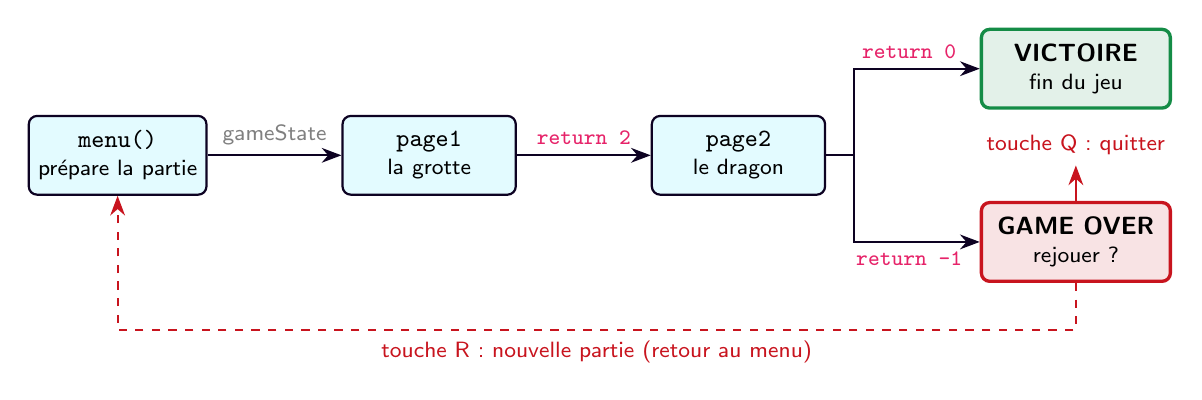
\begin{tikzpicture}[
    font=\small,
    boite/.style={draw=nuit, fill=pale!60, thick, rounded corners=3pt,
                  minimum width=2.2cm, minimum height=1cm, align=center},
    fin/.style={draw=#1, fill=#1!12, very thick, rounded corners=3pt,
                minimum width=2.4cm, minimum height=1cm, align=center, font=\small\bfseries},
    fleche/.style={-{Stealth[length=2.5mm]}, thick, nuit},
    etiq/.style={font=\ttfamily\footnotesize, text=magenta}
  ]
  \node[boite] (menu) {\texttt{menu()}\\[-1pt]{\footnotesize prépare la partie}};
  \node[boite, right=1.7cm of menu] (p1) {\texttt{page1}\\[-1pt]{\footnotesize la grotte}};
  \node[boite, right=1.7cm of p1] (p2) {\texttt{page2}\\[-1pt]{\footnotesize le dragon}};
  \coordinate[right=0.35cm of p2] (b);
  \node[fin=vert, anchor=west] (vic) at ($(b)+(1.6,1.1)$) {VICTOIRE\\[-1pt]{\footnotesize\mdseries fin du jeu}};
  \node[fin=rouge, anchor=west] (go) at ($(b)+(1.6,-1.1)$) {GAME OVER\\[-1pt]{\footnotesize\mdseries rejouer ?}};

  \draw[fleche] (menu) -- node[above, font=\footnotesize, text=gray]{gameState} (p1);
  \draw[fleche] (p1) -- node[etiq, above]{return 2} (p2);
  \draw[thick, nuit] (p2.east) -- (b);
  \draw[fleche] (b) |- node[etiq, pos=0.72, above]{return 0} (vic.west);
  \draw[fleche] (b) |- node[etiq, pos=0.72, below]{return -1} (go.west);
  \draw[fleche, dashed, rouge] (go.south) -- ++(0,-0.6) -| node[pos=0.25, below, font=\footnotesize, text=rouge]{touche R : nouvelle partie (retour au menu)} (menu.south);
  \draw[fleche, rouge] (go.north) -- ++(0,0.45) node[above, font=\footnotesize, text=rouge]{touche Q : quitter};
\end{tikzpicture}
\end{center}

Trois valeurs de retour sont spéciales :
\begin{itemize}
  \item \texttt{0} : le jeu se termine normalement (victoire, fin de l'histoire) ;
  \item \texttt{-1} : le joueur a perdu, l'écran GAME OVER s'affiche et propose de
        recommencer une partie (retour à \texttt{menu()}) ou de quitter ;
  \item \texttt{-2} : \textbf{cas non prévu}. C'est la valeur par défaut de vos pages
        (voir la convention \texttt{res} en partie~\ref{sec:consignes}). Si une page
        retourne \texttt{-2}, c'est que vous avez oublié un cas : le moteur s'arrête et
        vous indique la page en cause.
\end{itemize}

% ---------------------------------------------------------------------------
\section{Le dictionnaire \texttt{gameState}}

\texttt{gameState} contient tout ce dont votre jeu a besoin de se souvenir. C'est vous qui
choisissez ses clés dans \texttt{menu()}. Dans l'exemple fourni, \texttt{menu()} crée un
personnage ; dans votre jeu, elle peut faire tout autre chose. Les pages le lisent et le modifient directement :
les modifications sont conservées pour les pages suivantes, il n'y a \textbf{pas besoin de
le retourner}.

\begin{code}
# menu.py
def menu() -> dict:
    print("=== CRÉATION DU PERSONNAGE ===")
    nom: str = input("Quel est votre nom ? ")
    gameState: dict = {
        "nom": nom,
        "force": 7,
        "vie": 12,
        "inventaire": [],
    }
    return gameState      # menu() est la seule fonction qui retourne le dictionnaire
\end{code}

% ---------------------------------------------------------------------------
\section{Ajouter une page}

Pour ajouter la page 3 :
\begin{enumerate}
  \item créez le fichier \fichier{page3.py} dans votre dossier d'histoire ;
  \item écrivez dedans une fonction nommée \textbf{exactement} \texttt{page3}, qui prend
        un seul paramètre, \texttt{gameState}, et qui est \textbf{typée} :
        \texttt{def page3(gameState: dict) -> int:} ;
  \item première ligne de la fonction : \texttt{res = -2} ; dernière ligne :
        \texttt{return res} (c'est la convention \texttt{res}, voir
        partie~\ref{sec:consignes}) ;
  \item entre les deux, faites en sorte que \textbf{chaque cas} donne à \texttt{res} le
        numéro de la page suivante (ou \texttt{0} / \texttt{-1}) ;
  \item vérifiez qu'une autre page retourne bien \texttt{3}, sinon votre page ne sera
        jamais atteinte.
\end{enumerate}

\begin{code}
# page3.py
def page3(gameState: dict) -> int:
    res: int = -2              # par défaut : cas non prévu

    print("Deux couloirs s'ouvrent devant vous.")
    print("1 - Le couloir de gauche, d'où vient une odeur de soufre")
    print("2 - Le couloir de droite, plongé dans le noir")
    choix: str = input("> ")

    if choix == "1":
        res = 5
    elif choix == "2":
        gameState["vie"] = gameState["vie"] - 2
        print("Vous trébuchez dans le noir et perdez 2 points de vie.")
        if gameState["vie"] <= 0:
            res = -1           # plus de vie : GAME OVER
        else:
            res = 4
    else:
        print("Choix invalide.")
        res = 3                # on reste sur la même page

    return res
\end{code}

Si vous oubliez le \texttt{else} final et que le joueur tape autre chose que 1 ou 2,
\texttt{res} garde la valeur \texttt{-2} et le moteur vous le signale :

\begin{code}
ERREUR : La page 3 a retourné -2 : CAS NON PRÉVU.
\end{code}

\begin{astuce}[Les erreurs les plus fréquentes]
\begin{itemize}[leftmargin=1.2em]
  \item Le fichier s'appelle \fichier{page3.py} mais la fonction s'appelle \texttt{page\_3}
        ou \texttt{Page3} : les deux noms doivent être identiques.
  \item Un cas oublié (souvent le choix invalide) : \texttt{res} reste à \texttt{-2}.
  \item Le typage est oublié ou incomplet : le moteur refuse de lancer la page et vous
        rappelle la signature attendue.
  \item La page retourne \texttt{"4"} (du texte) au lieu de \texttt{4} (un nombre).
        Si le numéro vient d'un \texttt{input()}, convertissez-le avec \texttt{int(...)}.
  \item Une page appelle directement une autre page (\texttt{page4(gameState)}) au lieu
        de donner son numéro à \texttt{res} (\texttt{res = 4}).
\end{itemize}
\end{astuce}

% ---------------------------------------------------------------------------
\section{Ajouter un dessin en ASCII art}

Les dessins sont rangés dans le dossier \fichier{ASCII}, un dessin par fichier.
Le fichier \fichier{ascii\_dragon.py} sert de modèle.

\begin{enumerate}
  \item Copiez \fichier{ascii\_dragon.py} dans le dossier \fichier{ASCII} sous un nouveau
        nom commençant par \fichier{ascii\_}, par exemple \fichier{ascii\_tresor.py}.
  \item Renommez la fonction pour qu'elle porte \textbf{le même nom que le fichier} et
        gardez le typage : \texttt{def ascii\_tresor() -> None:}.
  \item Collez votre dessin entre les triple guillemets du \texttt{print}.
        \textbf{Gardez le \texttt{r} devant les guillemets} : sans lui, Python interprète
        mal les barres obliques inversées (\texttt{\textbackslash}) du dessin.
  \item Testez le dessin seul : \texttt{python ASCII/ascii\_tresor.py}.
\end{enumerate}

\begin{code}
# ASCII/ascii_tresor.py
def ascii_tresor() -> None:
    print(r"""
      ________
     /       /|
    /_______/ |
    |  $$$  | |
    |_______|/
""")
\end{code}

Pour l'afficher dans une page, importez la fonction en haut du fichier de la page, puis
appelez-la :

\begin{code}
# page5.py
from ASCII.ascii_tresor import ascii_tresor


def page5(gameState: dict) -> int:
    res: int = -2

    ascii_tresor()
    print("Vous découvrez un coffre rempli de pièces d'or !")
    gameState["inventaire"].append("or")
    res = 6

    return res
\end{code}

% ---------------------------------------------------------------------------
\section{Écrire des fonctions annexes}

Certaines actions reviennent souvent dans une histoire : un combat, un marchand, un
lancer de dé\dots{} Plutôt que de recopier le même code dans plusieurs pages, écrivez-le
une seule fois dans une \textbf{fonction annexe}, rangée dans le dossier
\fichier{OUTILS}. Contrairement aux pages, un fichier du dossier \fichier{OUTILS} peut
contenir \textbf{plusieurs fonctions}.

Le fichier \fichier{OUTILS/combat.py} vous est fourni comme exemple. Il contient :
\begin{itemize}
  \item une fonction générique \texttt{combat(gameState, monstre)}, où \texttt{monstre}
        est un dictionnaire (\texttt{"nom"}, \texttt{"vie"}, \texttt{"force"}). Elle
        retourne \texttt{True} (type \texttt{bool}) si le joueur gagne, \texttt{False} sinon.
        \textbf{Son contenu est à écrire par vous} ;
  \item des fonctions spécialisées, \texttt{combat\_dragon(gameState)} et
        \texttt{combat\_orc(gameState)}, qui créent chacune leur monstre puis appellent
        \texttt{combat}.
\end{itemize}

\begin{code}
# OUTILS/combat.py
def combat(gameState: dict, monstre: dict) -> bool:
    res: bool = False

    # A IMPLEMENTER

    return res


def combat_dragon(gameState: dict) -> bool:
    monstre: dict = {"nom": "dragon", "vie": 20, "force": 4}
    res: bool = combat(gameState, monstre)
    return res
\end{code}

Pour ajouter un monstre, écrivez une nouvelle fonction
sur le modèle de \texttt{combat\_dragon}.

Dans une page, importez la fonction puis utilisez son résultat
pour choisir la suite :

\begin{code}
# page2.py
from ASCII.ascii_dragon import ascii_dragon
from OUTILS.combat import combat_dragon


def page2(gameState: dict) -> int:
    res: int = -2

    ascii_dragon()
    print("Un dragon surgit et vous barre la route !")
    if combat_dragon(gameState):
        res = 0      # victoire
    else:
        res = -1     # GAME OVER

    return res
\end{code}

\begin{attention}[Seules les pages choisissent la page suivante]
Une fonction annexe retourne une \textbf{information} (gagné ou perdu, un objet
trouvé, une somme d'argent\dots), \textbf{jamais un numéro de page}. C'est toujours la
page qui décide de la suite, à partir de cette information.
\end{attention}

% ---------------------------------------------------------------------------
\newpage
\section{Consignes à respecter}\label{sec:consignes}

\begin{consignes}
\large
Un projet qui ne respecte pas ces consignes \textbf{ne fonctionnera pas avec le moteur}
et sera pénalisé.
\normalsize\raggedright
\begin{enumerate}[leftmargin=1.6em, label=\textbf{\color{rouge}\arabic*.}, itemsep=0.5em]
  \item \textbf{Ne modifiez jamais} \fichier{moteur.py} ni \fichier{ASCII/ascii\_gameover.py}.
  \item Ne renommez pas et ne déplacez pas les fichiers fournis. Seul le dossier
        \fichier{histoire\_A12} doit être renommé avec l'identifiant de votre équipe.
  \item \textbf{Un fichier par page.} Le fichier \fichier{pageX.py} contient
        \textbf{une seule fonction}, nommée \textbf{exactement} \texttt{pageX}, avec
        \textbf{un seul paramètre} : \texttt{gameState}.
  \item \fichier{menu.py} contient la fonction \texttt{menu()}, \textbf{sans paramètre},
        qui \textbf{retourne un dictionnaire}.
  \item Chaque page \textbf{retourne toujours un nombre entier} : le numéro d'une page qui
        existe, \texttt{0} pour la fin du jeu, \texttt{-1} pour le GAME OVER.
        \textbf{Appliquez les conventions} décrites dans l'encadré qui suit
        (un seul \texttt{return}, typage, pas de \texttt{break}).
  \item Une page \textbf{n'appelle jamais} une autre page : elle retourne son numéro.
  \item \textbf{Toutes vos fonctions sont typées}, paramètres et valeur de retour
        comprises : \texttt{def menu() -> dict:},
        \texttt{def page4(gameState: dict) -> int:}. Le moteur refuse une fonction non
        typée.
  \item Toutes les informations du jeu sont stockées dans \texttt{gameState}.
        \textbf{Aucune variable en dehors des fonctions}, pas de variables globales.
  \item Un fichier de page ne contient \textbf{rien d'autre} que sa fonction et,
        éventuellement, les \texttt{import} de vos dessins (\fichier{ASCII}) et de vos
        fonctions annexes (\fichier{OUTILS}).
  \item Les fonctions annexes sont rangées dans \fichier{OUTILS} et ne retournent
        \textbf{jamais} un numéro de page.
  \item Chaque dessin est dans \fichier{ASCII/ascii\_nom.py} et contient une fonction
        \texttt{ascii\_nom()}, sans paramètre.
  \item \textbf{Avant de rendre votre travail}, lancez
        \texttt{python moteur.py histoire\_XXX} et parcourez \textbf{tous les chemins}
        de votre histoire, y compris les choix invalides. Le jeu ne doit afficher aucun
        message d'erreur.
\end{enumerate}
\end{consignes}

\begin{convention}{CONVENTIONS : \texttt{res}, TYPAGE, PAS DE \texttt{break}}
\raggedright
\textbf{\color{magenta}1. Un seul \texttt{return} par fonction (la variable \texttt{res})}

Toutes vos fonctions qui retournent une valeur s'écrivent sur le même modèle :
\begin{itemize}[leftmargin=1.4em]
  \item \textbf{première ligne} : créez la variable \texttt{res} (pour \guil{résultat}) et
        donnez-lui une \textbf{valeur par défaut} ;
  \item \textbf{dernière ligne} : \texttt{return res}, et c'est le \textbf{seul}
        \texttt{return} de la fonction ;
  \item \textbf{entre les deux} : assurez-vous que, dans chaque cas, \texttt{res} reçoit
        la bonne valeur.
\end{itemize}

\begin{minipage}[t]{0.50\linewidth}
\begin{code}
def page7(gameState: dict) -> int:
    res: int = -2

    # chaque cas : res = ...

    return res
\end{code}
\end{minipage}\hfill
\begin{minipage}[t]{0.46\linewidth}\raggedright
\textbf{Valeurs par défaut :}
\begin{itemize}[leftmargin=1.2em]
  \item pages : \textbf{\texttt{-2}} (cas non prévu, le moteur affiche une erreur) ;
  \item fonctions annexes : une valeur adaptée à ce qu'elles retournent
        (\texttt{False}, \texttt{0}, \texttt{""}\dots).
\end{itemize}
\end{minipage}

\medskip
\textbf{\color{magenta}2. Tout est typé}

Indiquez le type de chaque paramètre et celui de la valeur retournée, ainsi que le type
des variables importantes. Les types utiles ici : \texttt{int}, \texttt{float},
\texttt{str}, \texttt{bool}, \texttt{list}, \texttt{tuple}, \texttt{dict}, et
\texttt{None} pour une fonction qui ne retourne rien (un dessin ASCII, par exemple).

\begin{code}
def page7(gameState: dict) -> int:
    res: int = -2
    choix: str = input("> ")
    ...
    return res
\end{code}

\medskip
\textbf{\color{magenta}3. Une boucle s'arrête uniquement par sa condition}

\texttt{break}, \texttt{continue} et \texttt{while True} sont interdits. La condition
écrite en haut du \texttt{while} doit dire, à elle seule, quand la boucle s'arrête.
Par exemple, pour redemander un choix tant qu'il n'est pas valide :

\begin{code}
choix: str = input("> ")
while choix != "1" and choix != "2":
    print("Choix invalide.")
    choix = input("> ")
\end{code}

\medskip
\textbf{\color{magenta}Pourquoi ces conventions ?}

Ce sont des \textbf{choix pédagogiques}, pas des règles universelles de la
programmation : un développeur expérimenté utilise parfois \texttt{break} ou plusieurs
\texttt{return}, en connaissance de cause, et Python n'oblige pas à typer. \textbf{Dans ce TP, elles sont en revanche
obligatoires.} Les respecter coûte en général une ou deux lignes de code, mais vous
oblige à réfléchir à la logique de votre programme avant de l'écrire : c'est exactement
ce que nous cherchons à vous faire acquérir.
\end{convention}

\newpage
\subsection{Notions interdites}

Ce TP est un exercice d'initiation. Vous devez utiliser \textbf{uniquement les notions vues
en cours} : variables, types de base, \texttt{input} / \texttt{print}, conditions
(\texttt{if} / \texttt{elif} / \texttt{else}), boucles (\texttt{for}, \texttt{while}),
fonctions, listes, tuples et dictionnaires. En particulier, les éléments suivants sont
\textbf{interdits} :

\begin{tcolorbox}[enhanced, colback=white, colframe=rouge!70, boxrule=1pt, arc=3pt]
\begin{minipage}[t]{0.48\linewidth}\raggedright
\begin{itemize}[leftmargin=1.2em]
  \item les classes et la programmation orientée objet (\texttt{class}, \texttt{self}) ;
  \item les variables globales (\texttt{global}, \texttt{nonlocal}) ;
  \item les fonctions \texttt{lambda} ;
  \item les listes ou dictionnaires en compréhension\newline
        (\texttt{[x for x in \dots]}) ;
  \item les exceptions (\texttt{try} / \texttt{except}, \texttt{raise}) ;
  \item l'instruction \texttt{match} / \texttt{case} ;
  \item \texttt{break}, \texttt{continue} et \texttt{while True} (voir les conventions) ;
\end{itemize}
\end{minipage}\hfill
\begin{minipage}[t]{0.48\linewidth}\raggedright
\begin{itemize}[leftmargin=1.2em]
  \item les décorateurs (\texttt{@\dots}) et les générateurs (\texttt{yield}) ;
  \item l'opérateur \guil{morse} \texttt{:=} ;
  \item \texttt{*args}, \texttt{**kwargs} ;
  \item la lecture et l'écriture de fichiers (\texttt{open}, \texttt{with}) ;
  \item \texttt{exit()}, \texttt{quit()}, \texttt{sys.exit()} : ils arrêtent le moteur ;
  \item les bibliothèques externes (installées avec \texttt{pip}) ;
  \item tout \texttt{import} autre que vos fichiers \fichier{ASCII} et
        \fichier{OUTILS}, sauf accord de votre enseignant.
\end{itemize}
\end{minipage}
\end{tcolorbox}

En cas de doute sur une notion, \textbf{demandez à votre enseignant avant de l'utiliser}.
Vous devez être capables d'expliquer chaque ligne de votre code.

% ---------------------------------------------------------------------------
\newpage
\section{Utiliser l'IA intelligemment}\label{sec:ia}

Vous avez le droit d'utiliser une IA (ChatGPT, Gemini, Claude, Le Chat\dots), mais comme un
\textbf{professeur particulier}, pas comme quelqu'un qui fait le travail à votre place.
Une IA à qui on demande \guil{écris-moi la page 3} produira souvent du code qui utilise
des notions interdites, que vous ne saurez pas expliquer, et qui ne respecte pas les
consignes du moteur.

Utilisez-la plutôt pour :
\begin{itemize}
  \item comprendre une notion du cours (\guil{comment fonctionne un dictionnaire ?}) ;
  \item comprendre un message d'erreur ;
  \item vérifier votre raisonnement sur un petit exemple ;
  \item obtenir des exercices pour vous entraîner.
\end{itemize}

Pour que l'IA se comporte comme un tuteur adapté à ce TP, donnez-lui les instructions
ci-dessous. Vous pouvez les coller au début de chaque conversation, ou mieux, les
enregistrer une fois pour toutes : dans un \textbf{Gem} (Gemini), un \textbf{GPT
personnalisé} ou un \textbf{Projet} (ChatGPT), un \textbf{Projet} ou une \textbf{Skill}
(Claude), ou dans les \textbf{instructions personnalisées} de votre outil.

Ce prompt est aussi fourni dans le fichier \fichier{promptAcopierColler.txt}, à la racine
de l'archive : vous pouvez copier son contenu, ou simplement téléverser le fichier dans
votre outil.

\begin{tcolorbox}[enhanced, colback=nuit, colframe=magenta, coltext=pale,
                  boxrule=1.2pt, arc=3pt, fonttitle=\bfseries, coltitle=white,
                  colbacktitle=magenta, title={Prompt à copier-coller}, left=8pt, right=8pt]
\footnotesize\setlength{\parskip}{0.25em}
Tu es un tuteur de programmation Python pour un étudiant en initiation à la
programmation. Je réalise un TP : un jeu de type \guil{livre dont vous êtes le héros}
où chaque page est une fonction pageX(gameState) placée dans son propre fichier
pageX.py, qui retourne le numéro de la page suivante (0 pour la fin du jeu, -1 pour le
game over). gameState est un dictionnaire qui contient l'état du jeu. Un moteur fourni
par l'enseignant enchaîne les pages : je ne dois pas le modifier. Je peux aussi écrire
des fonctions annexes (par exemple des combats) qui retournent une information, jamais
un numéro de page.

Conventions imposées : toutes les fonctions sont typées (par exemple
def page3(gameState: dict) -> int:) ; chaque fonction commence par res = valeur par
défaut (-2 pour une page, qui signifie « cas non prévu ») et se termine par un unique
return res.

Règles que tu dois respecter :

1. Ne m'écris jamais le code de mes pages ni la solution complète d'un exercice. Aide-moi
à trouver par moi-même : explique la notion, pose-moi des questions, donne-moi des
indices progressifs.

2. Si tu donnes un exemple de code, il doit être court (moins de 10 lignes) et porter
sur un autre sujet que mon jeu.

3. Dans tous tes exemples, respecte ces conventions : fonctions et variables typées ;
un seul return par fonction, en dernière ligne (variable res) ; jamais de break,
continue ou while True, une boucle s'arrête uniquement par sa condition.

4. N'utilise que les notions suivantes : variables, types de base, input, print, if /
elif / else, boucles for et while, fonctions, listes, tuples, dictionnaires et
annotations de type simples (int, str, bool, float, list, tuple, dict, None).
N'utilise jamais :
classes, global, lambda, compréhensions de listes, try / except, match / case, yield,
décorateurs, :=, *args / **kwargs, exit / quit / sys.exit, fichiers, bibliothèques
externes. Si ma question nécessite une de ces notions, dis-le-moi et propose une solution sans elle.

5. Quand je te montre un message d'erreur, explique-moi ce qu'il signifie et aide-moi à
trouver la ligne en cause, sans corriger le code à ma place.

6. Explique simplement, avec des mots adaptés à un débutant, et vérifie que j'ai compris
en me posant une question à la fin de tes explications.

7. Si je te demande de faire mon travail à ma place, refuse gentiment et rappelle-moi
ces règles.
\end{tcolorbox}

\begin{attention}[Rappel]
Le code rendu doit être \textbf{le vôtre}. Vous pourrez être interrogés sur n'importe
quelle partie de votre projet : un code que vous ne savez pas expliquer sera considéré
comme non réalisé.
\end{attention}

\end{document}
